\documentclass[tikz]{standalone}
\begin{document}
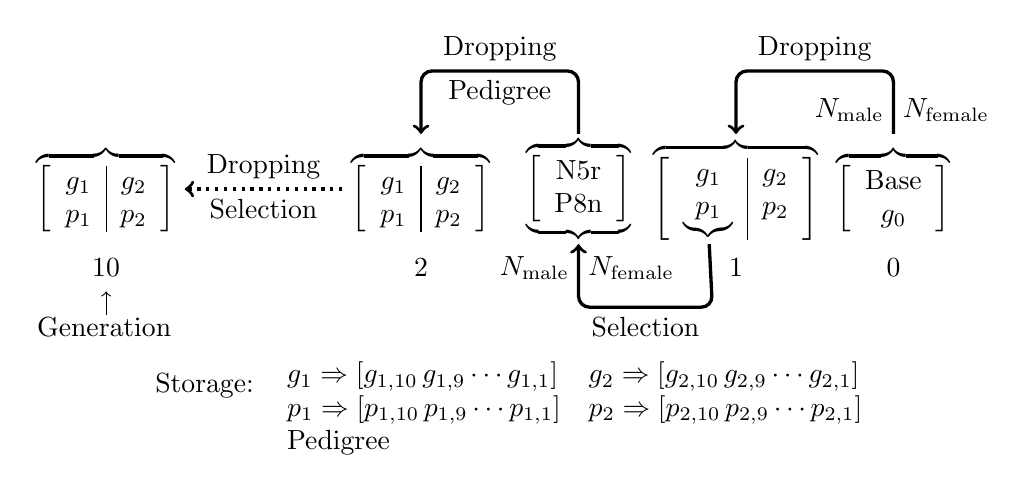
\begin{tikzpicture}
  %if to convert to jpg/png. but pdf is usually enougth.
  %convert -verbose -density 300 gs-data-structure.pdf -quality 100 -flatten -sharpen 0x1.0 t.jpg
  %\draw[help lines] (0,0) grid (12,5.5);
  %\foreach \x in {0, 1, ..., 11} \node[below, gray!50] at (\x,0){\tiny{\x}};
  %\foreach \y in {1, 2, ..., 6} \node[left, gray!50] at (0,\y){\tiny{\y}};
  \node at (11, 3.5) {$\overbrace{\left[\begin{array}{c}\mathrm{Base}\\
        g_0\end{array}\right]}$};
  \node at (11, 2.5) {0};
  \node at (9, 3.5) {$\overbrace{\left[\begin{array}{c|c}g_1 & g_2 \\
        \underbrace{p_1} & p_2 \end{array}\right]}$};
  \node at (9, 2.5) {1};
  \node at (7, 3.5) {$\overbrace{\underbrace{\left[\begin{array}{c}
            \mathrm{N5r}\\\mathrm{P8n}\end{array}\right]}}$};
  \node at (5, 3.5) {$\overbrace{\left[\begin{array}{c|c}g_1 & g_2 \\
        p_1 & p_2 \end{array}\right]}$};
  \node at (5, 2.5) {2};
  \node at (1, 3.5) {$\overbrace{\left[\begin{array}{c|c}g_1 & g_2 \\
        p_1 & p_2 \end{array}\right]}$};
  \node at (1, 2.5) {10};
  \node[right] at (0, 1.75) {Generation};

  \draw[->, very thick, rounded corners] (11,4.2)--(11,5)--(9,5)--(9,4.2);
  \node[right] at (11, 4.5) {$N_{\mathrm{female}}$};
  \node[left] at (11, 4.5) {$N_{\mathrm{male}}$};
  \node[above] at (10, 5) {Dropping};
  \draw[->, very thick, rounded corners] (8.66, 2.8)--(8.7, 2)--(7,2)--(7,2.8);
  \node[below] at (7.85, 2) {Selection};
  \draw[->, very thick, rounded corners, dotted] (4, 3.5)--(2, 3.5);
  \node[above] at (3, 3.5) {Dropping};
  \node[below] at (3, 3.5) {Selection};
  \draw[->] (1, 1.9)--(1, 2.2);
  \node[left] at (3, 1) {Storage:};
  \node[right] at (3, .7) {$\begin{array}{ll}
      g_1\Rightarrow[g_{1,10}\,g_{1,9}\cdots g_{1,1}] & g_2\Rightarrow[g_{2,10}\,g_{2,9}\cdots g_{2,1}]\\
      p_1\Rightarrow[p_{1,10}\,p_{1,9}\cdots p_{1,1}] & p_2\Rightarrow[p_{2,10}\,p_{2,9}\cdots p_{2,1}]\\
      \mathrm{Pedigree}
    \end{array}$};
  \draw[->, very thick, rounded corners] (7,4.2)--(7,5)--(5,5)--(5,4.2);
  \node[above] at (6, 5) {Dropping};
  \node[below] at (6, 5) {Pedigree};
  \node[right] at (7, 2.5) {$N_{\mathrm{female}}$};
  \node[left] at (7, 2.5) {$N_{\mathrm{male}}$};
\end{tikzpicture} 
\end{document}
